\documentclass[12pt,a4paper]{article}

% ---------------------------------------------------------------------------
% PACKAGES
% ---------------------------------------------------------------------------
\usepackage[T1]{fontenc}
\usepackage[utf8]{inputenc}
\usepackage[margin=2.5cm]{geometry}
\usepackage{lmodern}
\usepackage{microtype}
\usepackage{parskip}
\usepackage{booktabs}
\usepackage{tabularx}
\usepackage{graphicx}
\usepackage{float}
\usepackage{xcolor}
\usepackage{hyperref}
\usepackage{tikz}
\usetikzlibrary{positioning, arrows.meta, shapes.geometric, calc}

% Slightly more breathing room between paragraphs.
\setlength{\parskip}{0.75em}
\setlength{\parindent}{0pt}

\hypersetup{
	colorlinks=true,
	linkcolor=black,
	urlcolor=blue,
	citecolor=black
}

\title{Big Data: Search Engine Project\\Stage 1: Building the Data Layer}
\author{PIE data}
\date{Academic Year 2026/2027}

\begin{document}
	
	\pagenumbering{gobble}
	
	% ---------------------------------------------------------------------------
	% COVER
	% ---------------------------------------------------------------------------
	\begin{titlepage}
		\centering
		\vspace*{1.5cm}
		
		{\Large Universidad de Las Palmas de Gran Canaria\par}
		\vspace{0.3cm}
		{\large Grado en Ciencia e Ingeniería de Datos\par}
		
		\vspace{1.5cm}
		
		{\Huge\bfseries Big Data: Search Engine Project\par}
		\vspace{0.45cm}
		{\LARGE Stage 1: Building the Data Layer\par}
		
		\vspace{1.6cm}
		
		\begin{tabular}{ll}
			\textbf{Course:} & Big Data \\
			\textbf{Group:} & PIE data \\
			\textbf{Repository:} & \url{https://github.com/PIE-data/stage_1} \\
		\end{tabular}
		
		\vspace{1.6cm}
		
		{\large\bfseries Group members\par}
		\vspace{0.45cm}
		
		\begin{tabular}{l}
			Marcela Nieto-Kuczyńska \\
			Andrea Patruno \\
			Ivan Colella \\
			Manuel Muñoz Roca \\
		\end{tabular}
		
		\vfill
		{\large Academic Year 2026/2027\par}
	\end{titlepage}
	
	\clearpage
	\pagenumbering{roman}
	\tableofcontents
	\clearpage
	\pagenumbering{arabic}
	
	% ---------------------------------------------------------------------------
	\section{Introduction and Objectives}
	% ---------------------------------------------------------------------------
	The overall goal of the Big Data course project is to design and implement a simple
	search engine from scratch. Stage~1 focuses on the data layer: the part of the system
	responsible for acquiring documents, transforming them into consistent representations,
	storing them efficiently, and tracking the state of the pipeline.
	
	The dataset is based on Project Gutenberg. Each book is downloaded as plain text and
	split using the Project Gutenberg start and end markers into a header and a cleaned body.
	The header is used to extract structured metadata, while the body is tokenized to build
	a word-level inverted index. The footer is not required by the later search pipeline and
	is discarded.
	
	The objective of this stage is not only to build a working implementation, but also to
	compare alternative physical storage designs under controlled conditions. The pipeline is
	implemented in Python, Node.js, and Go, using the same corpora, normalization rules,
	workloads, and output contract in every language. This allows performance differences to
	be attributed to implementation and storage choices rather than to differences in
	functionality.
	
	The result of Stage~1 is a reliable and reproducible storage architecture that separates
	unstructured book content from structured, queryable data. A control layer makes the
	pipeline restartable and idempotent. This foundation will be reused in Stage~2 for
	ranking, phrase queries, and more advanced search functionality.
	
    % ---------------------------------------------------------------------------
	\section{System Architecture}
	\label{sec:architecture}
	% ---------------------------------------------------------------------------
	The system architecture is structured into three distinct physical and logical layers: the Datalake (raw artifact storage), the Datamarts (structured metadata and indices), and the Control Layer (state tracking and concurrency). The following diagram illustrates the data flow through the pipeline, from external ingestion to querying, with the control layer guiding the execution state.

	\begin{figure}[htbp]
		\centering
		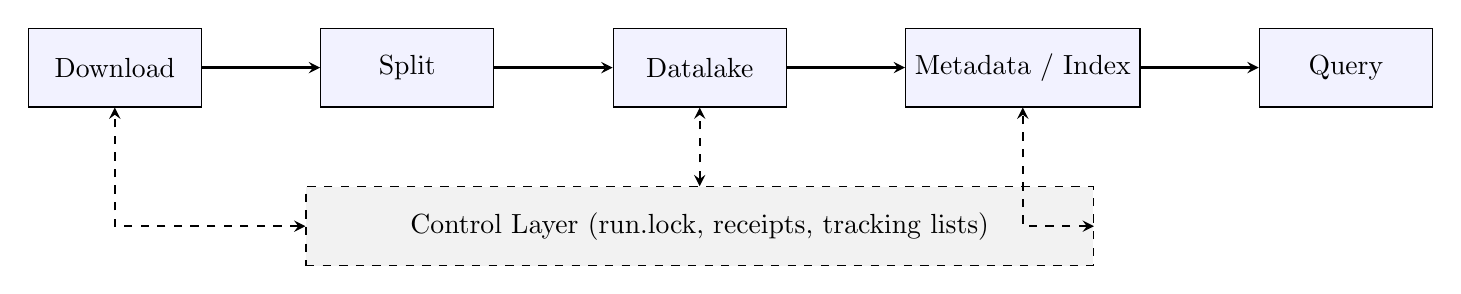
\begin{tikzpicture}[
			node distance=1cm and 1.5cm,
			box/.style={draw, rectangle, minimum width=2.2cm, minimum height=1cm, align=center, fill=blue!5},
			ctrl/.style={draw, dashed, rectangle, minimum width=10cm, minimum height=1cm, align=center, fill=gray!10},
			arrow/.style={->, >=stealth, thick}
		]

		% Main Pipeline
		\node[box] (download) {Download};
		\node[box, right=of download] (split) {Split};
		\node[box, right=of split] (datalake) {Datalake};
		\node[box, right=of datalake] (datamart) {Metadata / Index};
		\node[box, right=of datamart] (query) {Query};

		% Control Layer
		\node[ctrl, below=of datalake] (control) {Control Layer (run.lock, receipts, tracking lists)};

		% Pipeline Arrows
		\draw[arrow] (download) -- (split);
		\draw[arrow] (split) -- (datalake);
		\draw[arrow] (datalake) -- (datamart);
		\draw[arrow] (datamart) -- (query);

		% Control Interactions (Dashed)
		\draw[arrow, dashed, <->] (control.west) -| (download);
		\draw[arrow, dashed, <->] (control) -- (datalake);
		\draw[arrow, dashed, <->] (control.east) -| (datamart);

		\end{tikzpicture}
		\caption{System pipeline and Control Layer interaction.}
		\label{fig:pipeline}
	\end{figure}

	\subsection{Datalake}
	The Datalake stores the raw, split artifacts resulting from the ingestion of Gutenberg books. The system guarantees atomic writes for all artifacts and supports three mutually exclusive directory layouts:
	\begin{itemize}
		\item \textbf{Time-based layout:} Artifacts are partitioned by their UTC ingestion instant. The resulting paths are \texttt{datalake/<YYYYMMDD>/<HH>/<id>.body.txt} and \texttt{<id>.header.txt}.
		\item \textbf{Book-based layout:} Artifacts are grouped by book ID. The paths are \texttt{datalake/books/<id>/body.txt} and \texttt{header.txt}. Additionally, this layout stores a self-describing \texttt{meta.json} file alongside the text artifacts.
		\item \textbf{Hash-based layout:} Artifacts are sharded using the zero-padded 6-digit decimal representation of the book ID (\texttt{id6}). The paths isolate the first two and second two digits: \texttt{datalake/<id6[0:2]>/<id6[2:4]>/<id>.body.txt} and \texttt{<id>.header.txt}.
	\end{itemize}

	\subsection{Datamarts}
	The Datamarts transform the raw datalake files into structured queryable formats, separating metadata from the inverted index.

	\paragraph{Metadata Store.}
	The parsed header fields are stored in a centralized SQLite database located at \texttt{datamarts/metadata.db}. The database utilizes Write-Ahead Logging (WAL) and maintains a \texttt{books} table containing book identities, parsed author/title/language fields, paths relative to the workspace, file byte counts, and ingestion timestamps.

	\paragraph{Inverted Index Backends.}
	The inverted index records token frequencies and positional data for the document corpus. The architecture implements three interchangeable storage backends:
	\begin{itemize}
		\item \textbf{JSON (\texttt{json}):} A monolithic file at \texttt{datamarts/inverted\_index.json}. It acts as a single object mapping terms to their posting lists.
		\item \textbf{Folder (\texttt{folder}):} A distributed directory structure where each term operates as an independent file: \texttt{datamarts/inverted\_index/<BUCKET>/<safe\_term>.txt}. The bucket is the uppercase first character of the term (or \texttt{\_}), and the filename is percent-encoded to prevent case-collision on diverse filesystems.
		\item \textbf{SQLite (\texttt{sqlite}):} An embedded B-tree database at \texttt{datamarts/index.db} utilizing WAL mode. It contains a \texttt{terms} table for document frequencies and a \texttt{postings} table utilizing \texttt{WITHOUT ROWID} to store entries directly within the B-tree structure for optimization.
	\end{itemize}

	\subsection{Control Layer}
	The Control Layer strictly governs the execution state, pipeline resumption, and concurrency without relying on the physical presence of datalake artifacts. All control mechanisms reside within the \texttt{control/} directory:
	\begin{itemize}
		\item \textbf{State Tracking Lists:} \texttt{downloaded\_books.txt} and \texttt{indexed\_books.txt} maintain ascending, newline-separated lists of successfully processed book IDs. \texttt{failed\_books.txt} tracks unprocessable books alongside their error reasons (e.g., \texttt{NO\_MARKERS}).
		\item \textbf{Concurrency Lock:} \texttt{run.lock} provides a single-writer operating-system lock to safely prevent simultaneous modifications to the workspace by overlapping processes.
		\item \textbf{Ingestion Receipts:} Small JSON records written to \texttt{control/ingestion/<layout>/<id>.json}. They durably bind a book to its UTC ingestion instant (\texttt{ingested\_at}) and its definitive header and body paths.
	\end{itemize}
	
	% ---------------------------------------------------------------------------
	\section{Design Decisions}
	\label{sec:design}
	% ---------------------------------------------------------------------------
	Section~\ref{sec:architecture} describes \emph{what} the data layer contains; this
	section explains \emph{why}. Every decision was taken to make the comparison of
	Section~\ref{sec:benchmarks} fair first and fast second: three implementations that do
	not provably do the same work cannot be compared at all.

	\subsection{One Specification, One Oracle}

	All three implementations are written against a single specification,
	\texttt{docs/SPEC.md} (version~1.1.9). It fixes the command-line interface, the
	tokenizer, the header-parsing rules, the datalake layouts, the index and metadata
	formats and the exit codes. Every CLI refuses to run when its supported version differs
	from \texttt{spec/SPEC\_VERSION}, so a change to the specification cannot silently leave
	one language behind.

	Equivalence is checked, not assumed. Each implementation exports its inverted index in a
	\emph{canonical} form (JSON, UTF-8, no insignificant whitespace, terms in UTF-8 byte
	order, postings by ascending book id, positions ascending), and the SHA-256 of that
	export must equal a frozen value computed on 20 golden books. Continuous integration
	runs this \emph{conformance gate} for every language $\times$ index backend $\times$
	datalake layout: all 27 combinations produce the same hash. The metadata datamart is
	checked the same way during the benchmarks: the runner hashes every row that each
	language writes, and the three languages produce identical rows for every layout and
	corpus size.

	Two details of the canonical form exist only because of the other languages: terms are
	sorted by their UTF-8 bytes, because JavaScript's native string order (UTF-16) differs
	for characters outside the Basic Multilingual Plane; and Go's JSON encoder must not
	escape \texttt{<}, \texttt{>} and \texttt{\&}, which it does by default.

	\subsection{Programming Languages: Python, Node.js, and Go}

	Python is the reference implementation. Node.js and Go were chosen over Java because
	neither needs a build system to get started, and together the three cover the execution
	models we wanted to contrast: an interpreter (CPython), a just-in-time compiled runtime
	with an event loop (V8) and ahead-of-time compiled native code with lightweight threads
	(Go). The work was split by language on top of the shared specification, with one rule:
	nobody ported a component that affects the canonical hash and that they had written in
	Python, so that each port is an independent reading of the specification rather than a
	translation of the reference code. The rule was not kept everywhere: parts of the Node.js
	JSON backend and of the Go command-line wiring and index batching were completed by the
	author of the Python reference late in the project. Section~\ref{sec:benchmarks}
	lists this among the threats to validity.

	\subsection{Tokenization and Index Granularity}

	Text is normalised with NFKC, lower-cased independently of the locale and folded to
	ASCII where a mapping exists. Tokens are maximal runs of letters, digits and apostrophes;
	tokens shorter than 2 or longer than 40 code points, tokens made only of digits and
	English stop words are discarded. Positions are assigned \emph{before} filtering, so a
	gap between two positions marks a removed stop word.

	The index is word-level: for every term and book it stores the term frequency and the
	positions. This costs more space than a list of book ids, but it is what phrase queries
	and ranking functions such as TF-IDF or BM25 need in Stage~2.

	We deliberately do \textbf{not} stem. Stemming libraries in the three languages do not
	produce byte-identical output, which would break the conformance hash, and a
	hand-written stemmer in three languages was out of scope. For the same reason, regular
	expressions are allowed only to classify a single code point by Unicode category:
	regular-expression engines differ between languages precisely in the corners (Unicode
	classes, word boundaries) that decide where a token ends.

	\subsection{Corpus and Download}

	English books only, so that one stop-word list applies to the whole corpus. Fixed
	manifests of 100, 1\,000 and 10\,000 books (\texttt{spec/corpus/}) give a factor of ten
	between sizes; the measurements use 100 and 1\,000. Every benchmark downloads from a
	local HTTP mirror of Project Gutenberg: against the live site we would be measuring
	internet latency and its rate limiter, not our code.

	\subsection{Datalake Layouts}

	The three layouts trade lookup cost against the cost of finding new books:
	\begin{itemize}
		\item \textbf{time} groups books by ingestion hour. Finding the books ingested since a
		given instant only reads the folders from that hour on; looking up one book by id
		means searching every hour folder.
		\item \textbf{book} gives every book its own folder. Lookup is a direct path, and the
		folder can hold a self-describing \texttt{meta.json}; finding new books requires
		checking the modification time of every book.
		\item \textbf{hash} places a book in a two-level folder taken from the digits of its
		id, padded to six (\texttt{001342} $\rightarrow$ \texttt{00/13}). Lookup is a direct
		path and no folder holds more than 100 sub-folders, without one folder per book.
	\end{itemize}

	Every file is written atomically (temporary file, flush, \texttt{fsync}, rename,
	\texttt{fsync} of the parent folder), so a crash leaves either the old file or the new
	one, never half a book. In the benchmarks the time layout is filled at 100 books per
	hour: with a single ingestion instant every book would land in one folder and the layout
	would degenerate into a flat directory, which is not the structure being evaluated.

	\subsection{Inverted Index Backends}

	The three structures hold exactly the same information and differ only in how they
	store it: one large file (\textbf{json}), many small files (\textbf{folder}) and an
	embedded B-tree (\textbf{sqlite}).
	\begin{itemize}
		\item \textbf{json}: updating the index means reading, merging and rewriting the whole
		file. Incremental side files are forbidden by the specification precisely so that
		the update experiment measures that cost honestly.
		\item \textbf{folder}: one file per term, in 27 buckets (first letter, or \texttt{\_}).
		Term names are percent-encoded because raw terms collide as file names on
		case-insensitive file systems (NTFS, macOS) and on reserved names such as
		\texttt{CON}. Updating a book rewrites only the files of its terms.
		\item \textbf{sqlite}: postings live in a \texttt{WITHOUT ROWID} table keyed by
		\texttt{(term, book\_id)}, so the postings of a term are read from the primary-key
		tree itself with no second lookup; document frequency is kept in a separate
		\texttt{terms} table because every query reads it.
	\end{itemize}

	SQLite was preferred to MongoDB as the third structure: it needs no external service,
	its drivers are mature in all three languages, it is already used for the metadata
	datamart, and it turns the comparison into a clean axis --- one file, many files, one
	embedded B-tree --- instead of files versus a network server.

	\paragraph{Implementation choices that matter for the measurements.}
	Books are indexed in batches of 500: one rewrite of the JSON file, one rewrite of each
	touched term file and one SQLite transaction per batch, with document frequencies
	refreshed once per transaction for the terms touched. The JSON file holds exactly the
	canonical bytes in all three languages, so the three write the same amount of data.
	SQLite runs with a write-ahead log, \texttt{synchronous=NORMAL} and a 256~MiB page
	cache. None of these choices changes the content of the index --- the canonical hash is
	the same --- but they keep the measurements about the data structures rather than about
	avoidable overheads in our code; they are part of the specification, so every language
	follows them. The SQLite driver differs between languages: Python and Node.js use the C
	library, while Go uses \texttt{modernc.org/sqlite}, a translation of SQLite into Go that
	avoids a C compiler but is slower.

	\subsection{Metadata Datamart}

	Header fields are parsed into one SQLite table with indexes on author, language and
	title, the fields the benchmark queries filter on. The parsing rules are fixed in the
	specification because each of them caused a divergence between languages during
	development: fields start only at column~0 with a known name; an indented line continues
	the current field, and blank lines do not end it, because in some Gutenberg files the
	lines of a long field are separated by empty lines; the release date is a single line, and the
	indented ``Most recently updated'' line under it is ignored; month names come from a
	fixed English table, never from a locale-dependent date parser; languages are mapped to
	ISO~639-1 codes through a shared file.

	The ingestion instant of a book is recorded once, in a small receipt written when the
	book enters the datalake (\texttt{control/ingestion/<layout>/<id>.json}), and is the only
	source of the \texttt{ingested\_at} field. Rebuilding the metadata therefore always
	gives the same record, whatever the layout and whenever it is run, and the book
	layout's \texttt{meta.json} is written at ingestion time from the same record.

	Comparing alternative metadata stores is optional in the brief and was not done: the
	metadata stays in SQLite, and its build time and query time are measured instead.

	\subsection{Control Layer}

	The pipeline state lives in plain text files. A book is recorded as downloaded only
	after its files and its receipt are durable, and as indexed only after the batch
	containing it has been committed: a crash can therefore cause a book to be processed
	twice, never to be lost, and processing it twice is harmless because re-indexing
	replaces a book's postings instead of appending to them. \texttt{reconcile} rebuilds the
	control files from what is actually on disk, and an operating-system file lock prevents
	two runs on the same workspace --- a lock that disappears when the process dies, so a
	killed run can always be restarted. Each step of the control loop moves one book one
	stage forward, indexing pending books (smallest id first) before downloading the next
	one in manifest order, so the three languages process the same books in the same order.

	\subsection{How We Measure}

	Measurements are taken on two layers. The \emph{macro} layer runs each CLI command as a
	separate process, timed from outside with a monotonic clock, with peak memory taken by
	\texttt{/usr/bin/time} on the child process --- never self-reported --- so every
	language pays for its own runtime in the same way. Each command also reports its own
	internal time, which excludes interpreter start-up: for operations that take a few
	milliseconds, such as detecting new books, start-up (70--150~ms for Python) would
	otherwise be most of the number. The \emph{micro} layer times operations of micro- to
	milliseconds (lookup, index queries, metadata queries) inside the process with
	pytest-benchmark.

	Every configuration is run once as warm-up and then three times (the folder backend,
	which takes about ten minutes per run, without warm-up); the workspace is
	prepared outside the timer and the operating-system page cache is dropped before every
	measured run. We report medians and interquartile ranges rather than means, because
	background activity on a laptop produces occasional runs several times slower than the
	median.

	% ---------------------------------------------------------------------------
	\section{Benchmarks and Results}
	\label{sec:benchmarks}
	% ---------------------------------------------------------------------------
	\subsection{Dataset, Methods, and Measures}
	
	\begin{table}[H]
		\centering
		\caption{Benchmark design used for the Stage~1 evaluation.}
		\label{tab:dataset-method-measures}
		\small
		\begin{tabularx}{\textwidth}{p{0.20\textwidth} X X}
			\toprule
			\textbf{Dataset} & \textbf{Method} & \textbf{Measures} \\
			\midrule
			20-book golden corpus
			&
			Python, Node.js, and Go; all mandatory index backends
			&
			Canonical-export equality and conformance checks
			\\[0.4em]
			
			1,000-book English corpus
			&
			Language $\times$ datalake layout: time, book, batch/prefix
			&
			Download/write throughput; lookup latency; incremental-processing cost;
			recovery behavior; storage overhead
			\\[0.4em]
			
			1,000-book English corpus
			&
			Language $\times$ index backend: JSON, folder, SQLite
			&
			Indexing time; query latency; update time; peak RSS; on-disk size; file count
			\\[0.4em]
			
			100 / 1,000 / 10,000 books
			&
			Scaling runs for datalake layouts and index backends
			&
			Change in wall time, memory/disk footprint, and scalability trend
			\\
			\bottomrule
		\end{tabularx}
	\end{table}
	
	The benchmark protocol uses the same inputs and preprocessing rules for every language.
	Macro measurements time complete CLI commands from outside the process so that process
	startup and I/O are treated consistently. Short operations such as lookup and query are
	measured with language-specific micro-benchmark frameworks and normalized into a common
	metrics schema. Runs use a local mirror, a clean workspace, repeated measurements, and
	median/IQR summaries.
	
	\subsection{Results}
	
	\emph{TODO after the final benchmark run: insert the generated figures from
		\texttt{report/figures/} and discuss the measured differences between languages,
		datalake layouts, and index backends. The final text should identify the selected
		datalake layout and explain that choice using the benchmark results.}
	
	\subsection{Threats to Validity}
	
	The final interpretation should explicitly account for the fact that measurements are
	collected on one machine and one filesystem, the corpus is English-only, and even
	10,000 books remain modest compared with production-scale search systems. The local
	mirror intentionally removes internet variance, which improves repeatability but means
	that the benchmark does not measure real-world WAN behavior. Results are summarized over
	repeated runs, and the first run is treated as warm-up. SQLite is used as the third
	mandatory index structure instead of MongoDB, so conclusions about database-backed
	indexing are specific to an embedded relational store.
	
	% ---------------------------------------------------------------------------
	\section{Conclusions and Future Improvements}
	% ---------------------------------------------------------------------------
	Stage~1 establishes a common, reproducible data layer for the three implementations.
	The final conclusion should identify which datalake layout and inverted-index backend
	were selected after benchmarking and explain that choice using measured trade-offs
	rather than implementation preference alone.
	
	The positional index already contains document frequencies, term frequencies, and token
	positions needed by later search functionality. Stage~2 can therefore build ranking
	methods such as TF-IDF or BM25 and phrase-aware queries on top of the existing storage
	contract. Future work can also evaluate stemming, larger corpora, additional metadata
	backends, distributed storage, and a REST/API layer once the Stage~1 conformance and
	performance results are stable.
	
\end{document}